% Chapter 1

\chapter{555 Sampler Frequency } % Write in your own chapter title
\label{Chapter2}
\lhead{Chapter 2. \emph{555 Sampler Frequency}} % Write in your own chapter title to set the page header
\section{Description}
start with the following steps
\begin{itemize}
    \item Connect the circuit as shown in Figure 2.1.
    \begin{figure}[htbp]
	    \centering
	    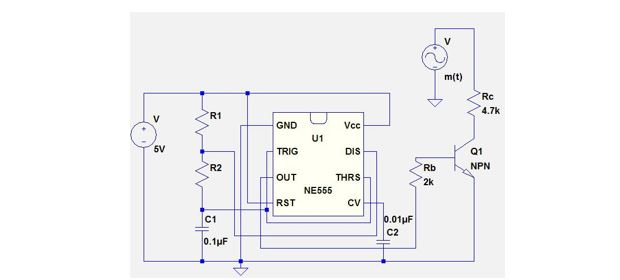
\includegraphics[width = 4in]{./Figures/sampler.jpg}
	    \rule{35em}{0.5pt}
	    \caption{Sampler using 555 Timer Circuit}
    \end{figure}
\end{itemize}
\begin{itemize}
    \item 555 timer is used to generate the switching sequence for the transistor which is operated in its saturation region. 555 timer is used in its astable mode as described above. The duty cycle of the output square wave is set to be much higher than 50\% to generate the sampled impulses at the output. This is in accordance with the Nyquist Sampling Theorem.

    \item The input to the transistor is shown in Figure 2.2.     
    \begin{figure}[htbp]
	    \centering
	    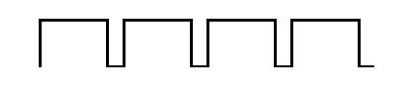
\includegraphics[width = 4in]{./Figures/input.jpg}
	    \rule{35em}{0.5pt}
	    \caption{input to the transistor}
    \end{figure}

    \item The time period of such an astable output is given by the sum of high time and low time. 
        \[T_H=0.7(R_1 + R_2) C_1\] 
        \[T_L=0.7*R_2*C_1\] 
    where T_H and T_L are high and low times, respectively.
\end{itemize}
\begin{itemize}
    \item Design 555 timer in astable mode so that duty cycle of the output waveform is 95\%. Use:
    \[C_1=0.1uF\]

    \item	The baseband signal m(t) is connected in series with the transistor. A dc component is added to m(t) to ensure that it remains positive. Negative values of m(t) cannot keep transistor in saturation mode. When transistor is OFF, m(t) appears at the output and when it is ON output voltage is zero. In this way m(t) is sampled.

    \item Keep the baseband signal amplitude to 2V and dc offset to 3V.

    \item Observe the sampled output on oscilloscope.
    \begin{figure}[htbp]
	    \centering
	    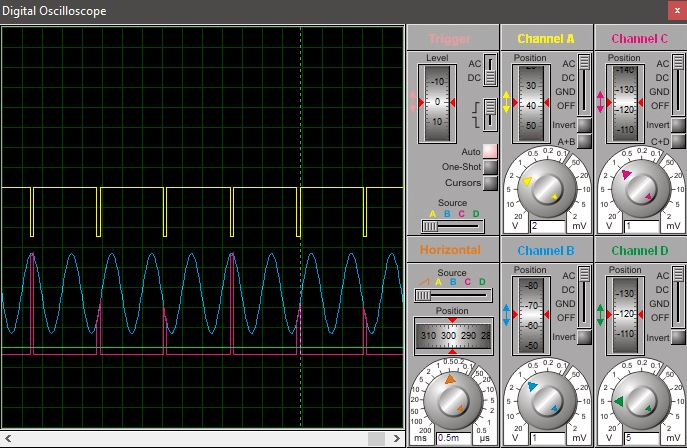
\includegraphics[width = 4in]{./Figures/general-output.jpg}
	    \rule{35em}{0.5pt}
	    \caption{Output of transistor without filter}
    \end{figure}
    
\end{itemize}

